% questions.tex —— 2015 年·北京卷·文科 · 题目内容片段（无答案）
% 由 tools/generate_projects.py 依来源总账自 2015/2015_数学真题_北京文_试题.md 生成，勿手改（改源 MD 后重跑）


\gkpart{数学}

\begin{gktip}
\textbf{来源说明}：本题面依据固定源 PDF 全 2 页逐题核对（p1＝页 937：栏 1 标题与「一、选择题」1–5、栏 2 6–14、栏 3 第 14 题图与 ①②＋「三、解答题」15–16；p2＝页 938：栏 1 解答 17–18、栏 2 解答 19、栏 3 解答 20）。原卷为 \textbf{A3 横向（1190.55 \(\times\) 841.89 pt）三栏书刊合排}，阅读序＝左→中→右；\textbf{页脚仅印合订本书页页码 937／938}（页面底部正中），\textbf{无页眉}。标题「2015 普通高等学校招生考试（北京卷文）」在栏 1 内排印。\textbf{全卷不印分值、不印题量、不印「考生注意」栏}——三处节头逐字仅「一、选择题」「二、填空题」「三、解答题」，解答题无「（本小题满分 N 分）」行；总分 150 为结构推断，\textbf{卷面无凭据}，本文件不作补写。

\textbf{源制作体系判定}（\texttt{pdffonts}／\texttt{pdftotext -layout}／\texttt{pdfimages -list} 实测）：源\textbf{不是扫描件，而是 LaTeX（Computer Modern 系）重排产物}——\texttt{pdfimages -list} 零命中（全页无位图；p1 117 条路径＝98 描边＋19 纯填充箭头，p2 64 条路径全描边）；嵌入字体含中文 \textbf{STSong（宋体正文）／STHeiti（黑体标题与节头）／STKaiti（仅第 8 题「注」行）}，拉丁与数学 \textbf{LMRoman 系与 CM 系（CMR10／CMMI10／CMSY10／MSAM10／CMMIB10 等）}。文本层整体可读；\textbf{「$\parallel$」两处为矢量描边绘制}（第 6 题、第 18 题 (1)，文本层完全缺失——按语义排印 \(\parallel\)）；根号上划线、表线、全部箭头亦为矢量路径。

\textbf{标点与字样约定（实测）}：① \textbf{题号与句末}源内为半角 \texttt{.}，按全库约定写作全角「．」；② \textbf{正文句读}源内为半角 ASCII（\texttt{, : ; ?}）与半角括号，本文件按全库约定归一为全角「，」「：」「；」「？」「（）」，\textbf{顿号「、」为全角 CJK·照源保留}，内容零改动；③ \textbf{选择题选项标号}源内为\textbf{半角「(A)」照录}；④ \textbf{作答空}：填空题为统一长度横线（实测 31.5 pt，写作 \texttt{\gkblank{}}），选择题作答括注按全库约定写作「（　）」；⑤ \textbf{分数}源内均为行间式样（真分式），排印一律按显示风格（如 \(\dfrac{a}{b}\)）；⑥ \textbf{不等号／集合／三角／角号}：不等号若出现按 MSAM10 排 \(\leqslant\)，\(\cap\)、\(\triangle\)、\(\angle\) 等按实测字形录入；⑦ \textbf{向量}：第 6 题的 \(\boldsymbol{a}\)、\(\boldsymbol{b}\) 源为\textbf{粗斜体}（CMMIB10），录作 \(\boldsymbol{a}\)／\(\boldsymbol{b}\)；⑧ \textbf{双曲线／椭圆等方程}照源；第 19 题 (2) 区间右端点的 \(\mathrm{e}\) 源为\textbf{正体拉丁}，录作 \(\sqrt{\mathrm{e}}\)；⑨ \textbf{表格}：全卷 3 张有线框 tabular（第 4 题 5\(\times\)2、第 8 题 3\(\times\)3、第 17 题 7\(\times\)5）——本文件按本库制表规范以 booktabs 三线表录入（内容逐格照源；第 17 题表头斜线分栏录作「顾客人数＼商品」）；⑩ \textbf{词间空格}照页面词界补，公式内部间距交数学模式自动还原。

\textbf{存疑与登记}（源内异常一律照录；完整清单见工作档 \texttt{page-map.md} §7 与 \texttt{figure-inventory.md} 存疑表 S-1…S-13）：① \textbf{第 14 题两幅散点图与题干不完全对应}——题干称「某班 37 位学生」，但左幅（语文）实绘 \textbf{35 点}、右幅（数学）实绘 \textbf{37 点}，两幅横坐标集合互不相同（独立生成、无一一对应）；「甲」「乙」仅见于左幅、「丙」仅见于右幅——系源重排产物特征，\textbf{照源复刻}，第 ② 小问按「总成绩名次」为公共键的跨图定位法读出（见答案）；② 第 17 题表内 \(\surd\)／\(\times\) 的行归属在文本层不可判（词盒顶偏移 9.6／4.9 pt ＞ 行高 15.51 pt），终端判格以字形墨迹中心为准（已双路复核，(217,丁) 格为 \(\surd\)）；③ 第 6 题与第 18 题 (1) 的「$\parallel$」为矢量描边（右倾双斜线），文本层静默丢失，按语义排印；④ 第 4 题「某」字在内容流中以字面串写出（CID 0x0D2A），已按字节还原核对；⑤ 第 8 题「注」行源用楷体（全卷唯一），系源排字样、不影响内容。
\end{gktip}

\gkpart{试题}

\gkpart{一、选择题}

\begin{question}
\gkti{1}若集合 \(A=\{x\mid -5<x<2\}\)，\(B=\{x\mid -3<x<3\}\)，则 \(A\cap B=\)（　）

(A) \(\{x\mid -3<x<2\}\)　(B) \(\{x\mid -5<x<2\}\)

(C) \(\{x\mid -3<x<3\}\)　(D) \(\{x\mid -5<x<3\}\)

\end{question}
\begin{question}
\gkti{2}圆心为 \((1,1)\) 且过原点的圆的方程是（　）

(A) \((x-1)^{2}+(y-1)^{2}=1\)　(B) \((x+1)^{2}+(y+1)^{2}=1\)

(C) \((x+1)^{2}+(y+1)^{2}=2\)　(D) \((x-1)^{2}+(y-1)^{2}=2\)

\end{question}
\begin{question}
\gkti{3}下列函数中为偶函数的是（　）

(A) \(y=x^{2}\sin x\)　(B) \(y=x^{2}\cos x\)

(C) \(y=|\ln x|\)　(D) \(y=2^{-x}\)

\end{question}
\begin{question}
\gkti{4}某校老年、中年和青年教师的人数见下表，采用分层抽样的方法调查教师的身体状况，在抽取的样本中，青年教师有 \(320\) 人，则该样本中的老年教师人数为（　）

\begin{center}
\begin{tabular}{ll}
\toprule
类别 & 人数 \\
\midrule
老年教师 & 900 \\
中年教师 & 1800 \\
青年教师 & 1600 \\
合计 & 4300 \\
\bottomrule
\end{tabular}
\end{center}

(A) \(90\)　(B) \(100\)　(C) \(180\)　(D) \(300\)

\Needspace{0.4\textheight}
\end{question}
\begin{question}
\gkti{5}执行如图所示的程序框图，输出 \(k\) 的值为（　）
\nopagebreak[4]
\begin{center}% 第 5 题程序框图：按固定源内容流矢量层精确值复刻（1 pt → 0.03515 cm，与全库同制）。
% 原点取框图竖轴 x=233.4258 pt、底缘 y（顶向下）=764.9258 pt；y 向上。
% 源实测：7 框（开始/结束=圆角 27.988 宽、框2=矩形 96.348×28.063 含真分式、框3 37.148×13.555、
% 框4 50.656×15.160、菱形 126.215×31.430、输出=平行四边形（斜偏 6.1328））；
% 6 段竖直连接 + 「否」支 3 段直角回边（左行 19.836、上行 80.930、右行 79.641，箭头落 框2/框3 之间竖线上）。
\begin{tikzpicture}[x=0.03515cm,y=0.03515cm,>=stealth,every node/.style={font=\small,inner sep=0pt},
  gl/.style={line width=0.398bp,line cap=round,line join=round}]
% ===== 7 框 =====
\draw[gl,rounded corners=0.1401cm] (-13.9961,209.6367) rectangle (13.9922,226.4688);   % 1 开始
\draw[gl] (-48.1758,167.0078) rectangle (48.1718,195.0703);                            % 2 k=0,a=3,q=1/2
\draw[gl] (-18.5742,138.8868) rectangle (18.5742,152.4414);                            % 3 a=aq
\draw[gl] (-25.3281,109.1602) rectangle (25.3281,124.3203);                            % 4 k=k+1
\draw[gl] (63.1055,78.7969)--(0,94.5117)--(-63.1094,78.7969)--(0,63.0821)--cycle;      % 5 菱形 a<1/4
\draw[gl] (-24.7774,31.5781)--(-18.6446,48.4297)--(24.7695,48.4297)--(18.6367,31.5781)--cycle; % 6 输出 k
\draw[gl,rounded corners=0.1401cm] (-13.9961,0) rectangle (13.9922,17.0117);           % 7 结束
% ===== 竖直连接（6 段，均 x=0）=====
\draw[gl,->] (0,209.4375)--(0,195.2696);   % 开始→框2
\draw[gl,->] (0,166.8125)--(0,152.6446);   % 框2→框3
\draw[gl,->] (0,138.6875)--(0,124.5196);   % 框3→框4
\draw[gl,->] (0,108.9610)--(0,94.7930);    % 框4→菱形顶
\draw[gl,->] (0,62.8008)--(0,48.6328);     % 菱形底→框6
\draw[gl,->] (0,31.3789)--(0,17.2110);     % 框6→结束
% ===== 「否」回边（3 段直角折线 + 箭头，落 框2/框3 之间竖线）=====
\draw[gl,->] (-63.3906,78.7969)--(-83.2266,78.7969)--(-83.2266,159.7266)--(0,159.7266);
% ===== 框内文字与分支标签（照源字形包围盒中心定位）=====
\node at (0,218.5358) {开始};
\node at (0,181.0390) {\(k=0,\ a=3,\ q=\dfrac{1}{2}\)};
\node at (0,146.9200) {\(a=aq\)};
\node at (0,116.0158) {\(k=k+1\)};
\node at (0,78.0860) {\(a<\dfrac{1}{4}\)};
\node at (-0.0800,40.1658) {输出 \(k\)};
\node at (0,8.9358) {结束};
\node at (-63.3258,87.6058) {否};
\node at (9.0342,56.2358) {是};
\end{tikzpicture}
\end{center}
\nopagebreak[4]
(A) \(3\)　(B) \(4\)　(C) \(5\)　(D) \(6\)

\end{question}
\begin{question}
\gkti{6}设 \(\boldsymbol{a}\)，\(\boldsymbol{b}\) 是非零向量，“\(\boldsymbol{a}\cdot\boldsymbol{b}=|\boldsymbol{a}||\boldsymbol{b}|\)”是“\(\boldsymbol{a}\parallel\boldsymbol{b}\)”的（　）

(A) 充分而不必要条件　(B) 必要而不充分条件

(C) 充分必要条件　(D) 既不充分也不必要条件

\Needspace{0.4\textheight}
\end{question}
\begin{question}
\gkti{7}某四棱锥的三视图如图所示，该四棱锥最长棱的棱长为（　）
\nopagebreak[4]
\begin{center}% 第 7 题三视图：按固定源内容流矢量层精确值复刻（1 pt → 0.03515 cm，与全库同制）。
% 原点取正视图左下顶点（源页 (517.1250, 198.8984) pt），y 向上；三幅足尺 62.3398 pt = 1 单位。
% 源实测：正视图＝直角三角形（直角在右下）、侧视图＝同向直角三角形（直角亦在右下，非镜像）、
% 俯视图＝正方形＋自右下至左上的一条实线对角线；三组「双向箭头+端刻度线」尺寸标注（数字 1）；
% 全图无虚线、无填充（除 6 个尺寸箭头）。题注括号按全库先例用全角。
\begin{tikzpicture}[x=0.03515cm,y=0.03515cm,>=stealth,every node/.style={font=\small,inner sep=0pt},
  gl/.style={line width=0.398bp,line cap=round,line join=round}]
% ===== 三幅轮廓 =====
\draw[gl] (0,0)--(62.3398,0)--(62.3398,62.3398)--cycle;            % 正（主）视图（直角右下）
\draw[gl] (93.5117,0)--(155.8516,0)--(155.8516,62.3398)--cycle;     % 侧（左）视图（同向）
\draw[gl] (0,-93.5078)--(62.3398,-93.5078)--(62.3398,-31.1680)--(0,-31.1680)--cycle; % 俯视图
\draw[gl] (62.3398,-93.5078)--(0,-31.1680);                        % 俯视图对角线
% ===== 尺寸标注（a）正视图宽度 y=-6.2344 =====
\draw[gl] (0,-3.1172)--(0,-9.3516);
\draw[gl] (62.3398,-3.1172)--(62.3398,-9.3516);
\draw[gl,->] (24.9375,-6.2344)--(0,-6.2344);
\draw[gl,->] (37.4063,-6.2344)--(62.3398,-6.2344);
\node at (31.3800,-6.9666) {1};
% =====（b）侧视图宽度 =====
\draw[gl] (93.5117,-3.1172)--(93.5117,-9.3516);
\draw[gl] (155.8516,-3.1172)--(155.8516,-9.3516);
\draw[gl,->] (118.4453,-6.2344)--(93.5117,-6.2344);
\draw[gl,->] (130.9141,-6.2344)--(155.8516,-6.2344);
\node at (124.9200,-6.9666) {1};
% =====（c）竖向高度 x=68.5742（数字落在轴线断口）=====
\draw[gl] (65.4570,62.3398)--(71.6914,62.3398);
\draw[gl] (65.4570,0)--(71.6914,0);
\draw[gl,->] (68.5742,40.5234)--(68.5742,62.3398);
\draw[gl,->] (68.5742,21.8203)--(68.5742,0);
\node at (68.8000,30.4534) {1};
% ===== 三幅题注 =====
\node at (31.3750,-19.4266) {正（主）视图};
\node at (124.9250,-19.4266) {侧（左）视图};
\node at (31.3750,-100.6516) {俯视图};
\end{tikzpicture}
\end{center}
\nopagebreak[4]
(A) \(1\)　(B) \(\sqrt{2}\)　(C) \(\sqrt{3}\)　(D) \(2\)

\end{question}
\begin{question}
\gkti{8}某辆汽车每次加油都把油箱加满，下表记录了该车相邻两次加油时的情况

\begin{center}
\begin{tabular}{lll}
\toprule
加油时间 & 加油量 (升) & 加油时的累计里程 (千米) \\
\midrule
2015 年 5 月 1 日 & 12 & 35000 \\
2015 年 5 月 15 日 & 48 & 35600 \\
\bottomrule
\end{tabular}
\end{center}

注：“累计里程”指汽车从出厂开始累计行驶的路程．

在这段时间内，该车每 \(100\) 千米平均耗油量为（　）

(A) \(6\) 升　(B) \(8\) 升　(C) \(10\) 升　(D) \(12\) 升

\end{question}
\gkpart{二、填空题}

\begin{question}
\gkti{9}复数 \(\mathrm{i}(1+\mathrm{i})\) 的实部为\gkblank{}．

\end{question}
\begin{question}
\gkti{10}\(2^{-3}\)，\(3^{\frac{1}{2}}\)，\(\log_{2}5\) 三个数中最大的数是\gkblank{}．

\end{question}
\begin{question}
\gkti{11}在 \(\triangle ABC\) 中，\(a=3\)，\(b=\sqrt{6}\)，\(\angle A=\dfrac{2\pi}{3}\)，则 \(\angle B=\)\gkblank{}．

\end{question}
\begin{question}
\gkti{12}已知 \((2,0)\) 是双曲线 \(x^{2}-\dfrac{y^{2}}{b^{2}}=1\) \((b>0)\) 的一个焦点，则 \(b=\)\gkblank{}．

\Needspace{0.4\textheight}
\end{question}
\begin{question}
\gkti{13}如图，\(\triangle ABC\) 及其内部的点组成的集合记为 \(D\)，\(P(x,y)\) 为 \(D\) 中任意一点，则 \(z=2x+3y\) 的最大值为\gkblank{}．
\nopagebreak[4]
\begin{center}% 第 13 题线性规划图：按固定源内容流矢量层精确值复刻（1 pt → 0.03515 cm，与全库同制）。
% 原点取 O（源页 (545.1484, 728.8203) pt），y 向上；1 单位 = 31.1696 pt（足尺：C(0,2)、A(2,1)、B(1,0) 残差 ≤0.002）。
% 源实测：两轴带单向箭头、各向原点外伸出 15.58 pt；三角区域为闭合实线三角形（无填充、无刻度、无延长线）。
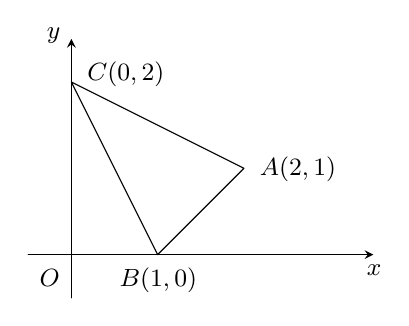
\begin{tikzpicture}[x=0.03515cm,y=0.03515cm,>=stealth,every node/.style={font=\small,inner sep=0pt},
  gl/.style={line width=0.398bp,line cap=round,line join=round}]
% ===== 坐标轴（单向箭头，照源顶点）=====
\draw[gl,->] (-15.5859,0)--(109.0938,0);   % x 轴
\draw[gl,->] (0,-15.5820)--(0,77.9258);    % y 轴
% ===== 三角区域（闭合实线）=====
\draw[gl] (0,62.3398)--(62.3399,31.1719)--(31.1680,0)--cycle;
% ===== 标签（照源字形包围盒中心定位）=====
\node at (-6.4434,79.1703) {\(y\)};
\node at (19.6966,65.3103) {\(C(0,2)\)};
\node at (81.8666,31.0103) {\(A(2,1)\)};
\node at (109.3416,-5.7647) {\(x\)};
\node at (-7.7934,-8.4197) {\(O\)};
\node at (31.3866,-9.1197) {\(B(1,0)\)};
\end{tikzpicture}
\end{center}
\nopagebreak[4]
\Needspace{0.4\textheight}
\end{question}
\begin{question}
\gkti{14}高三年级 \(267\) 位学生参加期末考试，某班 \(37\) 位学生的语文成绩、数学成绩与总成绩在全年级中的排名情况如图所示，甲、乙、丙为该班三位学生．
\nopagebreak[4]
\begin{center}% 第 14 题双散点图：按固定源内容流矢量层精确值复刻（1 pt → 0.03515 cm，与全库同制）。
% 原点取左幅 O（源页 (815.1758, 206.5898) pt），y 向上；右幅 O 在 x 偏移 +176.2461 pt。
% 坐标换算直接写在坐标表达式里（保留源页坐标可审计）：x_m = 页 x − O_x，y_m = 206.5898 − 页 y。
% 源实测：两幅各「左轴+下轴+右上直角折线框」130.914 × 130.914 pt（刻度端值 267，1 名次单位 = 0.490315 pt）；
% 散点 72 枚（左幅 35、右幅 37——源图与题干「37 位学生」不完全对应，照源复刻），字库 • 墨迹 2.45 pt；
% 标注：甲（左幅 (39.7,81.2) 点右）、乙（左幅 (126.6,67.5) 点右）、丙（右幅 (169.3,172.8) 点右）。
\begin{tikzpicture}[x=0.03515cm,y=0.03515cm,>=stealth,every node/.style={font=\small,inner sep=0pt},
  gl/.style={line width=0.398bp,line cap=round,line join=round}]
% ===== 左幅（语文）=====
\draw[gl,->] (0,0)--(149.6133,0);
\draw[gl,->] (0,0)--(0,149.6171);
\draw[gl] (130.9140,0)--(130.9140,130.9140)--(0,130.9140);
\node at (-11.2700,130.2400) {267};
\node at (131.2700,-7.8100) {267};
\node at (-7.6400,-8.2200) {\(O\)};
\node at (69.5300,-9.0500) {总成绩年级名次};
\node at (-8.6458,107.6200) {语}; \node at (-8.6458,97.0100) {文};
\node at (-8.6458,86.2700) {成}; \node at (-8.6458,75.4000) {绩};
\node at (-8.6458,64.5300) {年}; \node at (-8.6458,53.7400) {级};
\node at (-8.6458,42.9300) {名}; \node at (-8.6458,32.2200) {次};
\node at (28.7132,40.2998) {甲};
\node at (71.3702,33.4908) {乙};
\foreach \x/\y in {
816.2932/199.6777, 817.4135/154.7919, 817.4147/201.9215, 818.9112/204.9131,
819.2836/150.3038, 820.7801/101.3035, 823.7729/183.2193, 824.8945/134.2191,
826.0173/188.0817, 826.7646/127.1129, 830.8791/90.4566, 833.1234/145.0666,
834.6198/166.7616, 835.7414/150.3038, 839.1079/138.3335, 843.5978/187.7080,
844.7182/143.9450, 847.3380/182.0966, 848.4596/179.4785, 849.5812/97.1891,
851.0788/198.5549, 854.8172/141.3258, 860.4281/122.9985, 873.8942/147.3109,
876.1385/155.1661, 877.2595/173.4934, 877.6344/109.1593, 878.0080/130.8531,
889.9777/192.5698, 891.0999/141.3264, 896.7102/97.9388, 906.4355/102.0532,
906.8092/178.7300, 909.0535/203.0430, 913.1679/140.2048}
  \fill ({\x-815.1758},{206.5898-\y}) circle[radius=1.225];
% ===== 右幅（数学）=====
\draw[gl,->] (176.2461,0)--(325.8594,0);
\draw[gl,->] (176.2461,0)--(176.2461,149.6171);
\draw[gl] (307.1601,0)--(307.1601,130.9140)--(176.2461,130.9140);
\node at (165.0761,130.2400) {267};
\node at (307.5161,-7.8100) {267};
\node at (169.7061,-8.2200) {\(O\)};
\node at (246.8761,-9.0500) {总成绩年级名次};
\node at (167.7003,107.6200) {数}; \node at (167.7003,97.0100) {学};
\node at (167.7003,86.2700) {成}; \node at (167.7003,75.4000) {绩};
\node at (167.7003,64.5300) {年}; \node at (167.7003,53.7400) {级};
\node at (167.7003,42.9300) {名}; \node at (167.7003,32.2200) {次};
\node at (268.6382,85.2698) {丙};
\foreach \x/\y in {
992.9134/183.2189, 993.2883/194.0658, 993.6625/201.9211, 994.7841/204.1654,
995.9063/189.9514, 996.6542/200.4246, 997.7764/179.8524, 1000.3944/164.5168,
1002.2647/179.8524, 1002.2651/203.0426, 1003.3872/189.9514, 1008.6233/183.2189,
1010.4934/176.1116, 1011.9898/178.3560, 1013.4856/140.2038, 1016.1042/176.4853,
1019.8438/183.2189, 1022.8367/161.5239, 1023.5846/164.5168, 1026.2026/116.6399,
1026.2026/146.1883, 1026.5775/153.6687, 1028.4476/148.8063, 1031.0656/183.2189,
1038.1723/129.3569, 1052.3857/112.5255, 1053.8822/201.9211, 1055.0037/106.9146,
1055.0037/117.7615, 1056.5002/97.5629, 1068.8435/81.4794, 1069.2172/100.9294,
1074.4544/121.8753, 1082.3084/196.3102, 1084.5534/94.5706, 1087.9193/105.4175,
1092.0337/87.8382}
  \fill ({\x-991.4219+176.2461},{206.5898-\y}) circle[radius=1.225];
\end{tikzpicture}
\end{center}
\nopagebreak[4]
从这次考试成绩看，

① 在甲、乙两人中，其语文成绩名次比其总成绩名次靠前的学生是\gkblank{}；

② 在语文和数学两个科目中，丙同学的成绩名次更靠前的科目是\gkblank{}．

\end{question}
\gkpart{三、解答题}

\begin{question}
\gkti{15}已知函数 \(f(x)=\sin x-2\sqrt{3}\sin^{2}\dfrac{x}{2}\)．

（1） 求 \(f(x)\) 的最小正周期；

（2） 求 \(f(x)\) 在区间 \(\left[0,\dfrac{2\pi}{3}\right]\) 上的最小值．

\end{question}
\begin{question}
\gkti{16}已知等差数列 \(\{a_{n}\}\) 满足 \(a_{1}+a_{2}=10\)，\(a_{4}-a_{3}=2\)．

（1） 求 \(\{a_{n}\}\) 的通项公式；

（2） 设等比数列 \(\{b_{n}\}\) 满足 \(b_{2}=a_{3}\)，\(b_{3}=a_{7}\)，问：\(b_{6}\) 与数列 \(\{a_{n}\}\) 的第几项相等？

\end{question}
\begin{question}
\gkti{17}某超市随机选取 1000 位顾客，记录了他们购买甲、乙、丙、丁四种商品的情况，整理成如下统计表，其中“\(\surd\)”表示购买，“\(\times\)”表示未购买．

\begin{center}
\begin{tabular}{lllll}
\toprule
顾客人数＼商品 & 甲 & 乙 & 丙 & 丁 \\
\midrule
100 & \(\surd\) & \(\times\) & \(\surd\) & \(\surd\) \\
217 & \(\times\) & \(\surd\) & \(\times\) & \(\surd\) \\
200 & \(\surd\) & \(\surd\) & \(\surd\) & \(\times\) \\
300 & \(\surd\) & \(\times\) & \(\surd\) & \(\times\) \\
85 & \(\surd\) & \(\times\) & \(\times\) & \(\times\) \\
98 & \(\times\) & \(\surd\) & \(\times\) & \(\times\) \\
\bottomrule
\end{tabular}
\end{center}

（1） 估计顾客同时购买乙和丙的概率；

（2） 估计顾客在甲、乙、丙、丁中同时购买 3 种商品的概率；

（3） 如果顾客购买了甲，则该顾客同时购买乙、丙、丁中哪种商品的可能性最大？

\Needspace{0.4\textheight}
\end{question}
\begin{question}
\gkti{18}如图，在三棱锥 \(V-ABC\) 中，平面 \(VAB\perp\) 平面 \(ABC\)，\(\triangle VAB\) 为等边三角形，\(AC\perp BC\) 且 \(AC=BC=\sqrt{2}\)，\(O\)，\(M\) 分别为 \(AB\)，\(VA\) 的中点．
\nopagebreak[4]
\begin{center}% 第 18 题三棱锥 V-ABC：按固定源内容流矢量层精确值复刻（1 pt → 0.03515 cm，与全库同制）。
% 原点取 AB 中点 O（源页 (332.8438, 642.4805) pt），y 向上。
% 源实测：AB 水平长 113.3437（56.6719 pt/单位＝题设 2 单位）；△VAB 足尺等边（VA/VB 互差 ≤0.002、VO=98.1563＝√3/2·AB）；
% OC 为标准斜二测（左下 45°、深度折半 28.3312＝0.5 单位）；M 为 VA 中点（差 ≤0.0001）。
% 实线 6 条（VA、VB、VC、AC、BC、CM）；虚线 3 条（AB 被遮底棱、OM、OC）节距 2.98883/2.98883；无箭头、无填充。
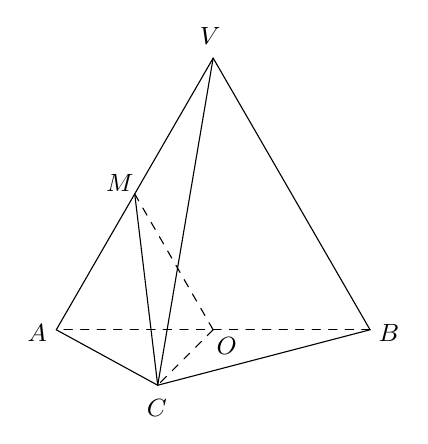
\begin{tikzpicture}[x=0.03515cm,y=0.03515cm,every node/.style={font=\small,inner sep=0pt},
  gl/.style={line width=0.3985bp,line cap=round,line join=round}]
% ===== 实线 6 条 =====
\draw[gl] (-56.6719,0)--(-20.0313,-20.0351);   % A→C
\draw[gl] (56.6718,0)--(-20.0313,-20.0351);    % B→C
\draw[gl] (0,98.1563)--(-56.6719,0);           % V→A
\draw[gl] (0,98.1563)--(56.6718,0);            % V→B
\draw[gl] (0,98.1563)--(-20.0313,-20.0351);    % V→C
\draw[gl] (-20.0313,-20.0351)--(-28.3360,49.0781); % C→M
% ===== 虚线 3 条（被遮棱与内部辅助线）=====
\draw[gl,dash pattern=on 2.98883pt off 2.98883pt] (56.6718,0)--(-56.6719,0);          % B→A
\draw[gl,dash pattern=on 2.98883pt off 2.98883pt] (0,0)--(-28.3360,49.0781);           % O→M
\draw[gl,dash pattern=on 2.98883pt off 2.98883pt] (0,0)--(-20.0313,-20.0351);          % O→C
% ===== 六顶点标签（照源字形包围盒中心定位）=====
\node at (-1.0388,106.0605) {\(V\)};
\node at (-33.7238,52.9255) {\(M\)};
\node at (-63.5388,-1.1045) {\(A\)};
\node at (63.5312,-1.1045) {\(B\)};
\node at (4.9112,-6.0345) {\(O\)};
\node at (-20.2888,-28.1195) {\(C\)};
\end{tikzpicture}
\end{center}
\nopagebreak[4]
（1） 求证：\(VB\parallel\) 平面 \(MOC\)；

（2） 求证：平面 \(MOC\perp\) 平面 \(VAB\)；

（3） 求三棱锥 \(V-ABC\) 的体积．

\end{question}
\begin{question}
\gkti{19}设函数 \(f(x)=\dfrac{x^{2}}{2}-k\ln x\)，\(k>0\)．

（1） 求 \(f(x)\) 的单调区间和极值；

（2） 证明：若 \(f(x)\) 存在零点，则 \(f(x)\) 在区间 \((1,\sqrt{\mathrm{e}}]\) 上仅有一个零点．

\end{question}
\begin{question}
\gkti{20}已知椭圆 \(C\)：\(x^{2}+3y^{2}=3\)，过点 \(D(1,0)\) 且不过点 \(E(2,1)\) 的直线与椭圆 \(C\) 交于 \(A\)，\(B\) 两点，直线 \(AE\) 与直线 \(x=3\) 交于点 \(M\)．

（1） 求椭圆 \(C\) 的离心率；

（2） 若直线 \(AB\) 垂直于 \(x\) 轴，求直线 \(BM\) 的斜率；

（3） 试判断直线 \(BM\) 与直线 \(DE\) 的位置关系，并说明理由．

\end{question}